\chapter{Results and Discussion}
This chapter presents the results of training the Explainable Boosting Machine (EBM) on the extracted linguistic
features from the I-JAS corpus. The section begins with an overview of the model's performance, followed by an
analysis of feature importance and concludes with a discussion of the results in light of previous findings and
methodological considerations.


\section{Model Performance}
%*Discuss f1, accuracy, precision
%*share confusion matrix
%*discuss small sample size for N1 group which likely affected the classification
%*could not achieve better than 50\% accuracy, probably due to the 5 groups and overlap between some proficiency
%levels. Still better performance than the 20\% random guess baseline....

The EBM was trained using the full set of extracted features on a five-class classification task corresponding to
the five JLPT proficiency levels (N5-N1). Interactions were set to zero to allow for clear interpretation of the
feature importances. The model was
evaluated using 5-fold cross-validation,
with oversampling to balance the minority classes (N1 and N5). The results, aggregated across all cross-validation
folds, are summarized
in Table~
\ref{tab:trainingResults}.


\begin{table}[h!]
    \centering
    \begin{tabular}{lcccc}
        \hline \textbf{Class} & \textbf{Precision} & \textbf{Recall} & \textbf{f1-score} & \textbf{Support} \\ \hline
        N5    &   0.45   &   0.51   &   0.48   &    735\\
          N4    &   0.43   &   0.39   &   0.41   &   1431\\
          N3    &   0.38   &   0.34   &   0.36  &    1342\\
          N2  &     0.34   &   0.38  &    0.36   &    816\\
          N1    &   0.15   &   0.19   &   0.17    &   224\\ \hline
        accuracy &   -    &      -    &     0.38  &    4548\\
   macro avg  &     0.35   &   0.36  &    0.35   &   4548\\
weighted avg  &     0.39  &    0.38    &  0.38   &   4548\\ \hline
    \end{tabular}
    \caption[Overall Classification Report (All Folds Combined)]{Overall Classification Report (All Folds Combined)}
    \label{tab:trainingResults}
\end{table}

The model achieved an overall accuracy of 38\%, demonstrating some capacity to distinguish between proficiency
levels.
While the overall performance did not exceed 50\%, it represents a significant improvement over a random guess
baseline of 20\% for a five-class classification problem. The F1-scores, which provide a harmonic mean of precision
and recall, ranged from 0.17 for N1 and 0.48 for N5 (Table~\ref{tab:trainingResults}).

Notably, classification performance declined as proficiency increased, with the N1 group showing the weakest
performance across all metrics (precision = 0.15, recall = 0.19, f1 = 0.17). This is likely attributable in part to the
small sample size of N1 texts in the corpus, as well as the overlap between the proficiency levels.

Performance was highest for the N5 and N4 levels, which may reflect the chosen features may be more robust against
distinguishing the lower proficiency and intermediate levels. In contrast, the model struggled to differentiate
adjacent intermediate levels N3-N2, which suggests a need for more sensitive or diversified features as shown in the
confusion matrix in Figure~\ref{fig:conMA}.

\begin{figure}[h!]
           \centering
           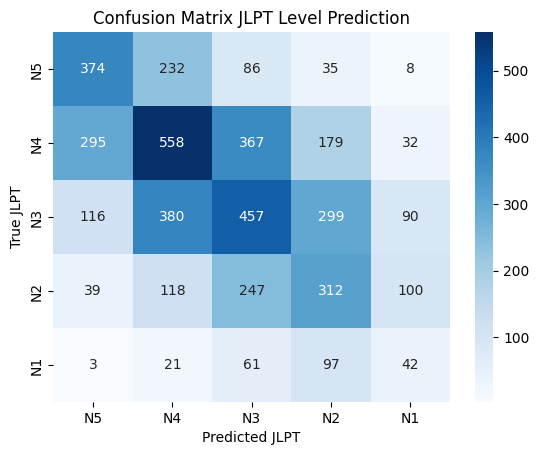
\includegraphics[scale=.4]{img/confusionMatrix}
           \caption[Confusion Matrix for JLPT Level Prediction]{Confusion Matrix for JLPT Level Prediction}
           \label{fig:conMA}
\end{figure}

A common misclassification was that a substantial number of true N3 instances were misclassified as N4(380) or N2 (
299).
Similarly, N2 texts were frequently predicted as N3 (245) or N1 (107), and N1 texts were often misclassified as N2 (
98) or N3 (62). This suggests that the model frequently confused text belonging to adjacent proficiency levels,
indicating a high overlap between the proficiency levels. This overlap was further supported when aggregating the
proficiency levels into three groups—Beginner (N5+N4),
Intermediate (N3+N2), and
Advanced (N1).
Classification performance for these three groups improved significantly, achieving an overall F1-score of 0.54. This
substantial increase from 0.38 F1-score for the five-class problem further corroborates the hypothesis that the
continuous nature of adjacent JLPT levels presents a significant challenge for fine-grained classification.

\section{Feature Importance Analysis}
\begin{figure}[h!]
    \centering
    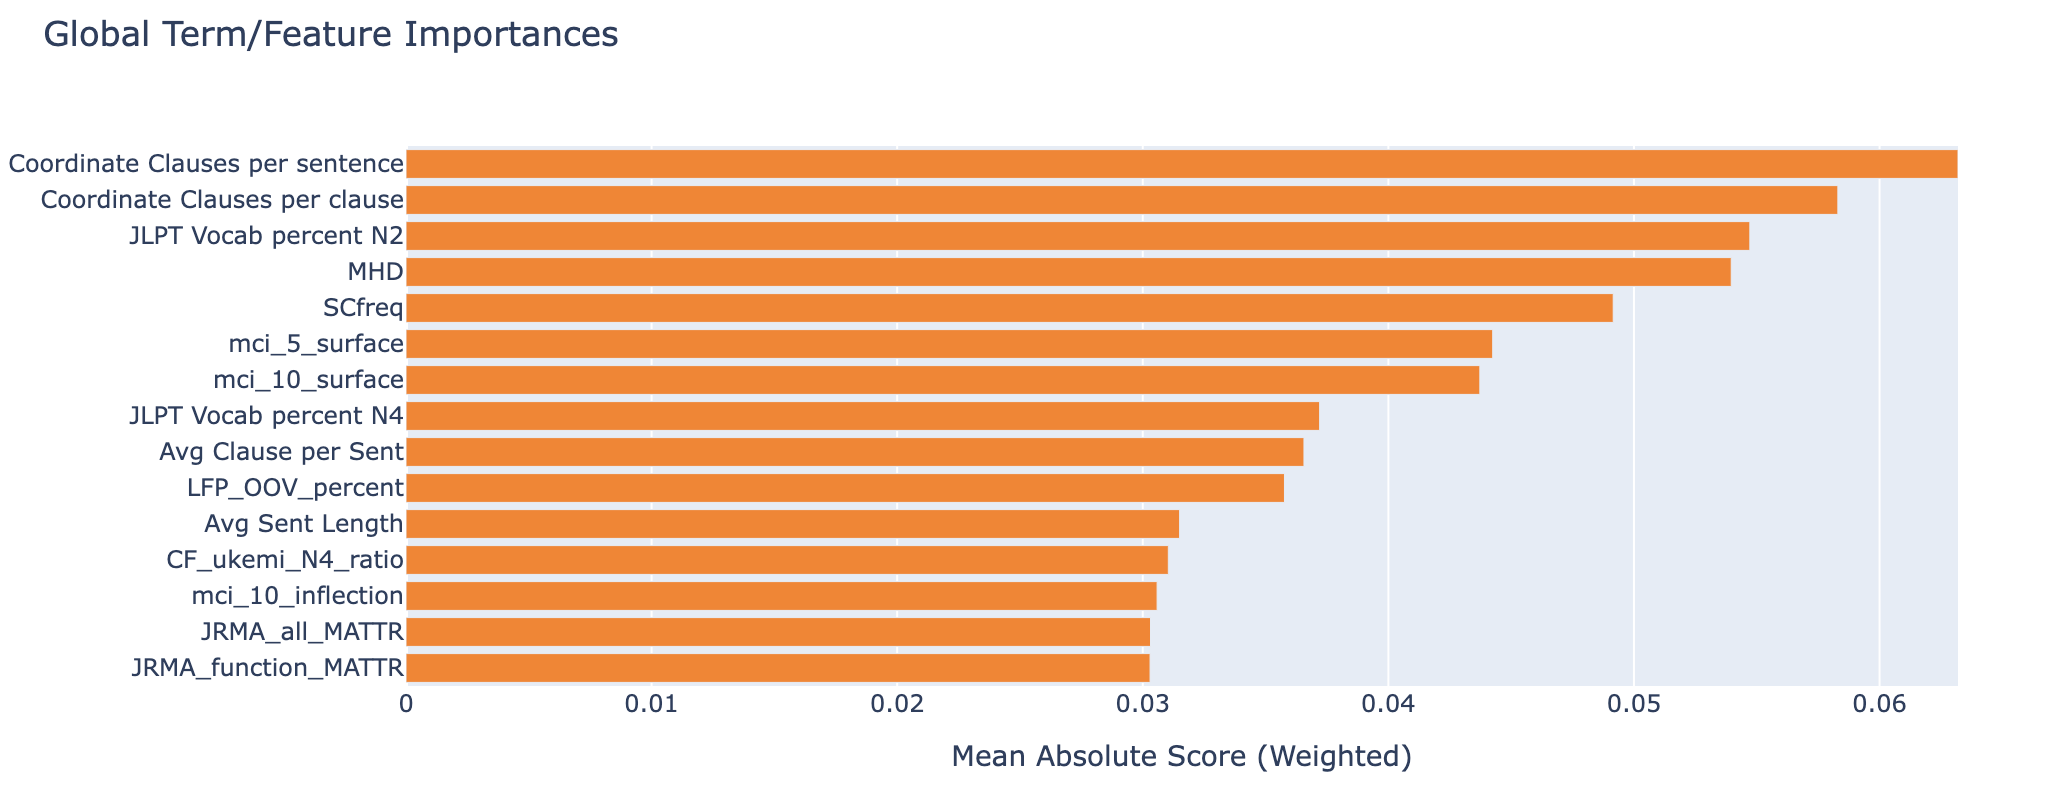
\includegraphics[scale=.4]{img/feature_importance}
    \caption[Feature Importance Chart]{ Feature Importance Chart: Top-ranked features contributing to the classification of JLPT proficiency levels, based on their additive contribution scores from the EBM model.}
    \label{fig:featureimportance}
\end{figure}


The feature importance results from the final EBM model are shown in Figure~\ref{fig:featureimportance}. A
more detailed chart showing the top 30 features with weights can be found in Appendix Table~\ref{tab:top30-importance}
Overall, a
diverse range of linguistic features contributed to classification accuracy, though complexity measures were most
prominent among the top-ranked features. A wide variety of complexity
measures, consisting of syntactic, lexical, and morphological contributed to classification, indicating that a
multidimensional approach is essential for classifying learner texts.

The top two features were coordinate clauses per sentence and coordinate clauses per clause, both measures of
syntactic complexity. These features suggest that the frequency of coordination structures is a strong
differentiator across proficiency levels, potentially a reflection of developmental gains in syntactic elaboration. This
aligns with findings in the previous section, where this feature was also found to discriminate between adjacent
levels in
the low to mid-proficiency ranges while also increasing at higher levels. The class
separation can be seen in Figure~\ref{fig:EBMccPerSent}, where N5 is associated with lower values (below 0.25),
while above 1 are associated with N1 and N2.


\begin{figure}[h!]
    \centering
    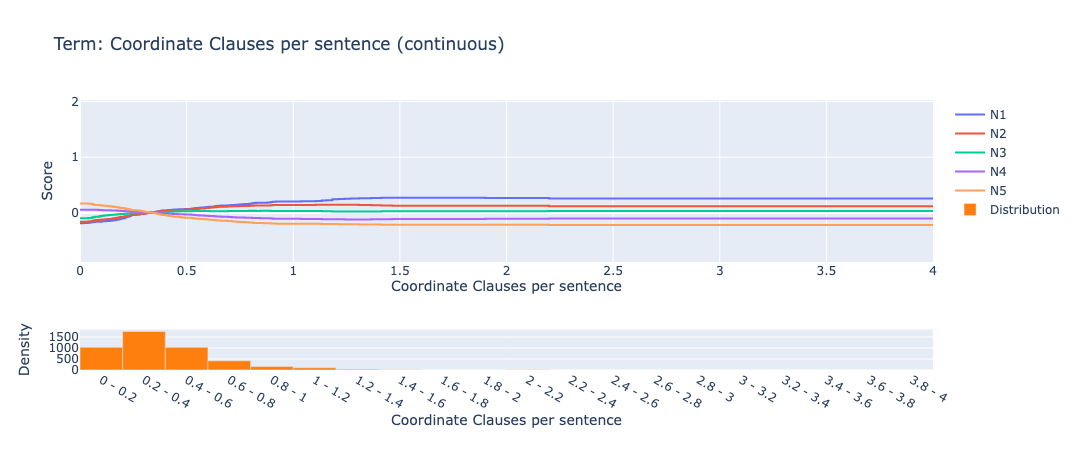
\includegraphics[scale=.4]{img/EBM/EBMccPerSent}
    \caption[Contribution of Coordinate Clauses per Sentence]{This chart represents how the feature of Coordinate clauses per sentence contributes to the prediction of each proficiency level}
    \label{fig:EBMccPerSent}
\end{figure}


The third-ranked feature, the ratio of words from JLPT N2 list to total tokens (Lexical Frequency Profile), highlights
lexical sophistication. A higher proportion of N2-level vocabulary
correlates with higher proficiency levels, consistent with previous lexical profiling studies\citep{Laufer1995}.
As shown in Figure~\ref{fig:EBMjlptN2}, this feature reliably distinguished between the N1 and N2 from the lower
levels.

\begin{figure}[h!]
    \centering
    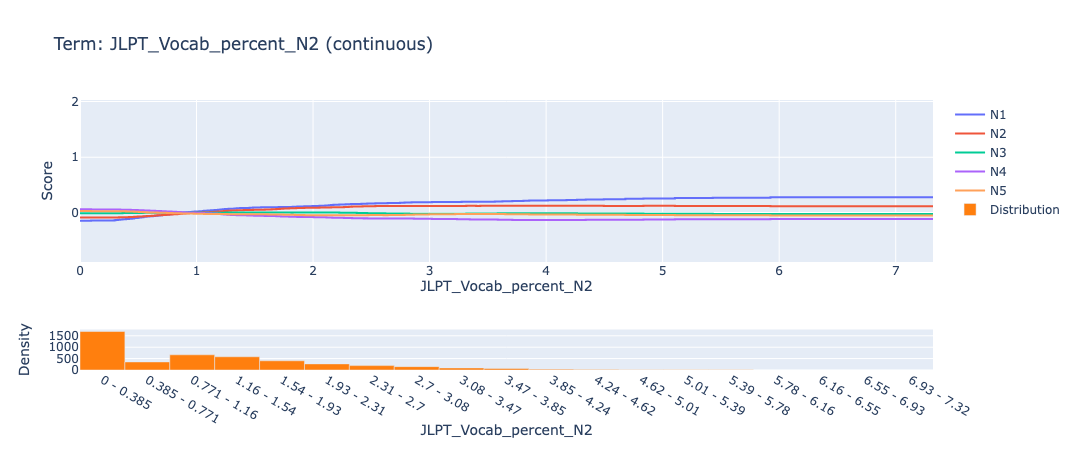
\includegraphics[scale=.4]{img/EBM/JLPTn2P}
    \caption[Contribution of percentage of tokens from JLPT N2 vocabulary list]{This chart shows how the percentage of tokens from JLPT N2 word list contributes to the prediction of each proficiency level}
    \label{fig:EBMjlptN2}
\end{figure}

Mean Hierarchical Distance (MHD), the fourth-ranked feature, quantifies the average depth of syntactic embedding.
Its presence in this list suggests that deeper syntactic constructions are a reliable signal for distinguishing the
higher proficiency levels.

Subordinate conjunction frequency (SCfreq), a proxy measure for subordination, was ranked fifth. This was somewhat
surprising, as lexical complexity measures such as Out of Vocabulary list (OOV) from the LFP were expected to be
more
predictive.
However,
due to the
tokenizer's tendency to misclassify coordinating conjunctions as subordinating ones, SCfreq may effectively capture
both types of clause-linking (coordination and subordination). Since coordination frequency was shown to increase
with proficiency, this blended feature still carries strong predictive value. Figure~\ref{fig:EBMSCfreq} shows its
role in distinguishing N5 from other levels, supported by a broad density range.

\begin{figure}[h!]
    \centering
    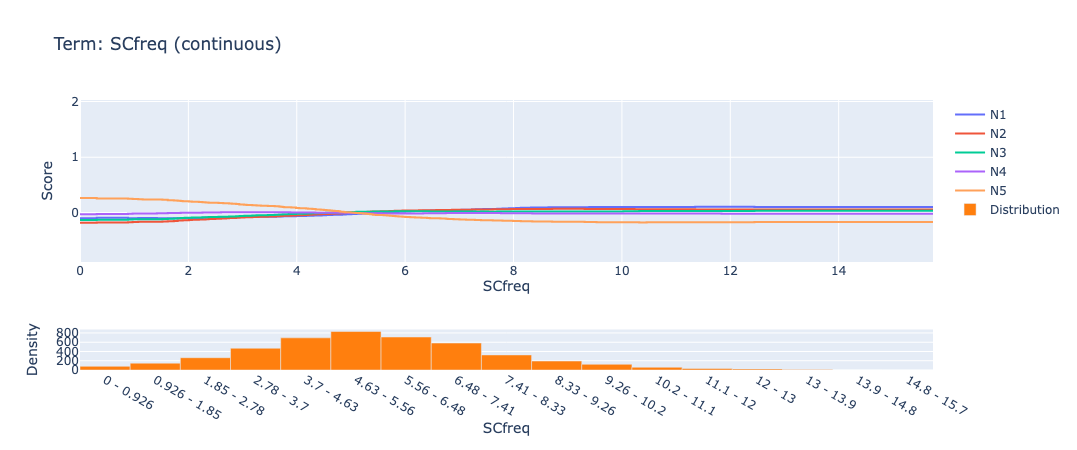
\includegraphics[scale=.4]{img/EBM/EBMSCfreq}
    \caption[Contribution of Subordinating Conjuction Frequency]{This chart shows how feature of Subordinating Conjunction frequency contributes to the prediction of each proficiency level}
    \label{fig:EBMSCfreq}
\end{figure}

Several morphological complexity indicators also appeared in the top features. Both MCI-5 surface and MCI-10
surface were ranked in the top ten, indicating that surface-level morphological diversity increases with
proficiency. Additionally, MCI-10 Inflection, which measures inflectional morphological diversity, was also
influential. This is notewrothy given that the larger text window used in its calculation excluded many shorter
texts. Although previously found to distinguish N1 from native speaker texts, Figure~\ref{fig:EBMMCI10inflection}
also shows that this feature contributes to differentiating within learner proficiency levels.

\begin{figure}[h!]
    \centering
    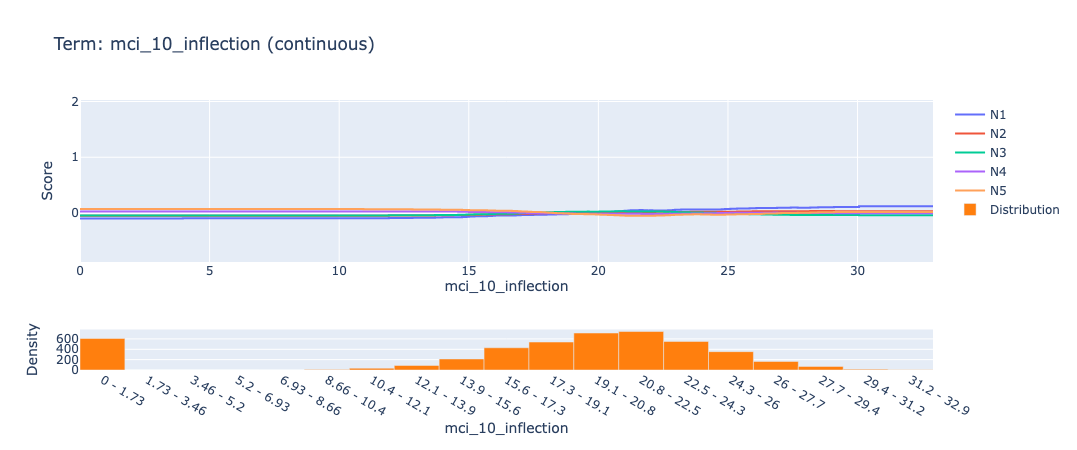
\includegraphics[scale=.4]{img/EBM/MCI10inflection}
    \caption[Contribution of MCI 10 Inflection measure]{This chart shows how the MCI10 inflection measure contributes to the prediction of each proficiency level}
    \label{fig:EBMMCI10inflection}
\end{figure}

JMRA Function MATTR and JMRA All MATTR also ranked among the top 15 as morphological diversity measures. This
suggests that variation in function, and all (function + content) morphemes, which also reflects grammatical
elaboration, is a
relevant factor in distinguishing between proficiency levels. As shown in Figure~\ref{fig:JMRAallMATTR}, higher
All MATTR
scores are associated with the advanced levels (N1 and N2), separating them from lower and intermediate groups.

\begin{figure}[h!]
    \centering
    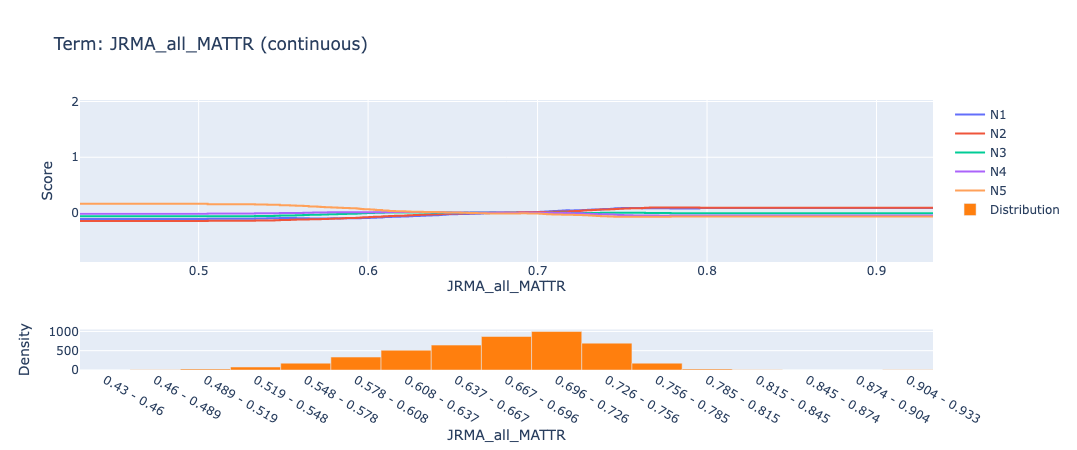
\includegraphics[scale=.4]{img/EBM/JMRAallMATTR}
    \caption[Contribution of JMRA function and content morphemes]{This chart shows how the feature of MATTR of content and function morphemes contributes to the prediction of each proficiency level}
    \label{fig:JMRAallMATTR}
\end{figure}

The proportion of tokens not included in the 10,000 word frequency list of the BCCJW corpus (LFP OOV Percent) was
also highly ranked in importance. This measure of lexical sophistication may signal either the use of advanced
vocabulary or the presence of unrecognized or erroneous forms. As shown in Figure~\ref{fig:EBMlfpOOV}, it
contributed most to distinguishing the lower proficiency levels (N5 and N4), possibly indicating the latter, as
there is a general decrease across proficency levels,
though
further investigation is needed.


\begin{figure}[h!]
    \centering
    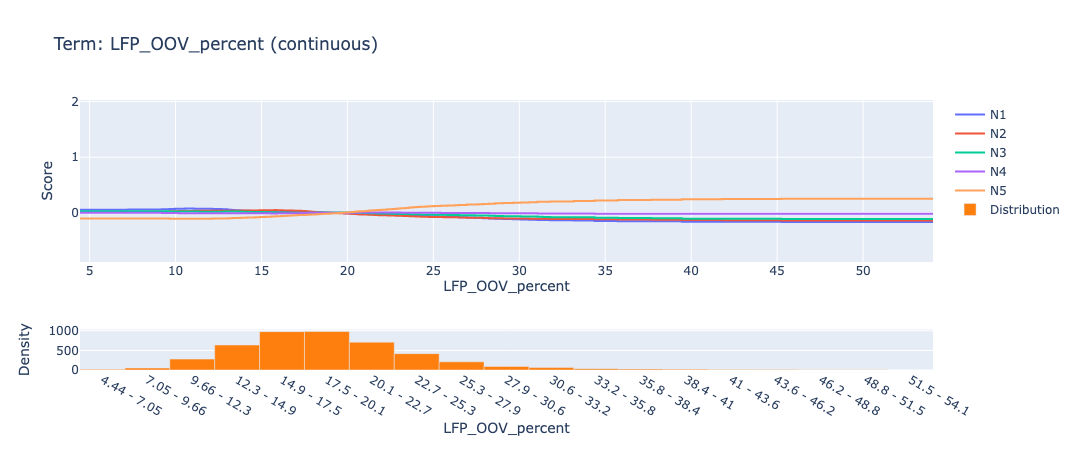
\includegraphics[scale=.4]{img/EBM/EBMlfpOOV}
    \caption[Contribution of Percentage of Lexical Frequency Profile (LFP)Out of Vocabulary (OOV) tokens]{This chart represents how the feature of Lexical Frequency Profile (LFP)Out of Vocabulary (OOV) tokens contributes to the prediction of each proficiency level}
    \label{fig:EBMlfpOOV}
\end{figure}


Only one criterial feature, Ukemi (受身形, passive voice), appeared among the top 15. Typically introduced to
learners at the N4 level, this form is often difficult to master, due to verb form transformation and unconventional
contexts which may differ from a learner's native language. The highest use of this form was at the N1 level. Figure~\ref{fig:EBMukemi} shows its ability to distinguish between levels, though low overall frequency limits its density and predictive power. Since the extractor only captures correct instances, incorporating incorrect uses could improve performance.

\begin{figure}[h!]
    \centering
    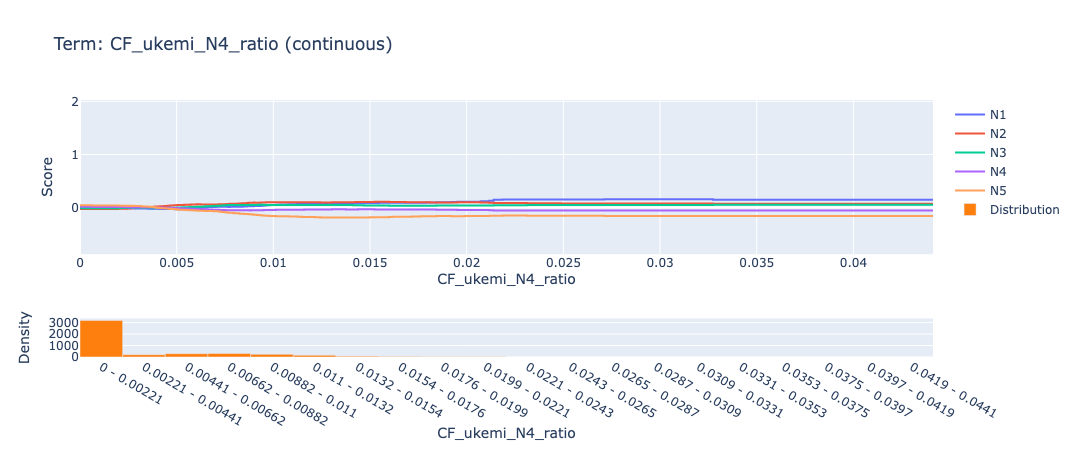
\includegraphics[scale=.4]{img/EBM/EBMukemi}
    \caption[Contribution of ratio of passive form (受身形、ukemi)]{This chart shows how the ratio of passive form to total tokens contributes to the prediction of each proficiency level}
    \label{fig:EBMukemi}
\end{figure}


Unsurprisingly, Sentence length was also among the top features. This was the only measure that consistently
distinguished between all JLPT levels and the native speaker group.

The EBM feature importance analysis confirms that no single metric defines learner proficiency. Rather, a
combination of syntactic elaboration, morphological diversity, and lexical distribution provides the strongest
predictive power.

\section{Discussion}

% Make conrete citations
The results above provide partial support for developmental patterns identified in the previous chapters. In
particular, some features showed a clear trajectory of increased usage of complexity across levels, supporting
earlier corpus based findings and previous literature. However the predictive power of many features was moderate,
as found in the f1 scores, and some expected distinctions between adjacent levels (e.g. N3 vs N2) were not captured
effectively.

This suggests that while form-based measures of grammatical complexity and frequency-based criterial features can be
useful, they may not be sufficient in isolation. Some grammatical forms exhibit nuanced usage that depends on
semantic, pragmatic, or discourse-level factors which are not easily captured through surface-form
analysis alone.

The model's diminished performance, particularly for N2 and N1 as evidenced by lower f1-scores and the high number
of misclassifications in the confusion matrix (Figure~\ref{fig:conMA}), points to inherent challenges in
classifying these adjacent proficiency levels. The significant overlap observed in predictions (e.g. N3 misclassified
as N2 and N4) suggests that the linguistic differences between intermediate and advanced levels are subtler and less
discretely based on the current feature set. It is plausible after all, that learners at adjacent intermediate
levels exhibit similar linguistic characteristics than, for example, a beginner (N5) and an advanced learner (N1).
This continuous nature of language development makes sharp categorical distinctions difficult for any model.

The small sample size of N1 group (44 participants, 224 texts) significantly impacted its classification accuracy (
F1-score
of 0.17 in Table~\ref{tab:trainingResults}). With fewer examples, the model had limited data to learn the specific
criteria that distinguish N1 texts from other levels, leading to a high rate of misclassification, particularly into
N2 and N3 categories. This data imbalance likely constrained the model's ability to fully capture the
characteristics of advanced learners.


\subsection{Limitations and Difficulties}
% integrate limitations from ch 4. into this section:
%One limitation of
%this analysis is that it is purely based on frequency of use and does not capture form-based errors. For forms like the
%passive construction (受身形), which require complex verb transformation and are introduced in later levels, analyzing
%accuracy and types of errors in their production could provide additional insight into learner
%acquisition patterns and developmental stages. Future research should aim to incorporate error analysis to provide a
%more comprehensive understanding of the mastery of grammar features. This would enable a more nuanced understanding
%of not just what forms learners use, but how correctly they use them at different stages of development. Further
%work could also investigate the influence of task genre on the frequency of these grammar forms. This is important
%as certain tasks might elicit specific forms, and understanding this relationship would help refine future corpus
%design attempts to control for these variables and extract specialized forms for more targed analysis.


The corpus, consisting of uncorrected learner language, posed challenges for feature extraction. Misspellings and
grammatical errors common in learner output could lead to incorrect tokenization and POS tagging by the underlying
NLP tools (e.g. SpaCy's GinZA package), thus impacting the accuracy of extracted features. For instance, irregular
forms or "mispellings" might be incorrectly counted as out-of-vocabulary words (in the context of the LFP complexity
measure), rather than as specific error types. More crucially, the morphological complexity of Japanese,
particularly with compound verbs and auxiliary constructions (e.g. 「言い切る」 as one verb vs. 「食べ切る」 parsed into two
parts), meant that rule-based feature extraction struggled with consistency. This could lead to undercounting or
categorising certain complex forms, which could be a critical indicator of advanced proficiency.

The variability in text length, with some texts being very short, likely affected the reliability of certain
density-based metrics. Such metrics are sensitive to text
length, and calculation over very short texts can yield less stable or representative values, potentially
introducing noise into the feature set.

While features like coordinate clauses per sentence were highly important, the accuracy of their extraction was
dependent on the underlying tokenizer's ability to correctly identify conjunctions and clause boundaries. As noted
previously, many Japanese conjunctions can be used in both coordinating and subordinating contexts, and rule-based
parsers like SpaCy may not fully account for contextual nuances. This potential inaccuracy in the input features
could directly limit the model's ability to use these syntactic measures for precise classification. A more robust,
context-aware parsing system would likely improve the accuracy of these measures.

The feature extractor largely focused on form-based grammatical constructs that are relatively easier to identify
programmatically and are common in standardized written Japanese. This approach may have overlooked more nuanced,
use-based grammatical patterns that could be highly discriminative of proficiency. Futhermore, the reliance on rules
for standardized written language means that variations due to dialects or highly casual written forms, if present
in the learner corpus, would not have been accurately captured, potentially missing valuable information for
classification.

A significant limitation of the current study was the exclusion of learner errors as a direct feature. Different
proficiency levels are often
characterized by distinct error patterns, as was illustrated in \citet{Hawkins_Buttery_2010}. The
developmental trajectory of errors, where specific error types and frequencies change systematically with
proficiency, could provide highly discriminative information for the model.
Incorporating
systematic error analysis as a
feature
set
could provide
highly discriminative information, potentially leading to substantial improvements in classification accuracy,
especially for distinguishing between adjacent intermediate and advanced levels where subtle error reductions or
shifts in error types might be useful indicators.

While these levels have been validated
\citet{jcat_interpretation_guide}, they
are primarily based on recognition tasks (reading and listening) and do not directly assess productive skills like
writing or speaking. Therefore, the proficiency labels assigned to the learner texts, derived from J-Cat, are approximations of a broader construct of proficiency. There can be considerable variance in the productive language capabilities of individuals who score similarly on the JLPT, which might introduce inherent 'noise' or ambiguity into the dataset, further complicating the task of classification for the model.

While the EBM demonstrated a capability to classify JLPT levels better than chance, it's performance highlights the
inherent
complexity of distinguishing between closely related proficiency levels in a continuous developmental spectrum. The
identified features were significant, but future improvements would benefit from addressing the methodological
challenges in feature extraction, particularly for nuanced Japanese linguistic structures, and exploring the
integration of error-based features.